\begin{center}
    \section*{Практична частина}
\end{center}

Для дослідження методів, описаних у теоритичнії
частині, нами, на мові программування Python, було імплементовано усі вищезазначені алгоритми,
а саме:
\vspace{0.25cm}
\begin{enumerate}
    \item Гука-Дживса
    \item Нелдера-Міда
    \item Метод Ньютона
    \item Квазіньютоновські методи:
    \begin{enumerate}
        \item SR1
        \item Broyden
        \item DFP
        \item BFGS
    \end{enumerate}
    \item Генетичний алгоритм
\end{enumerate}

За допомогою цих алгоритмів ми будемо шукати
рішення безумовної задачі оптимізації \ref{eq:optimization_task}
для наступних функцій:

\begin{figure}[h!]
    \begin{subfigure}{0.3 \textwidth}
        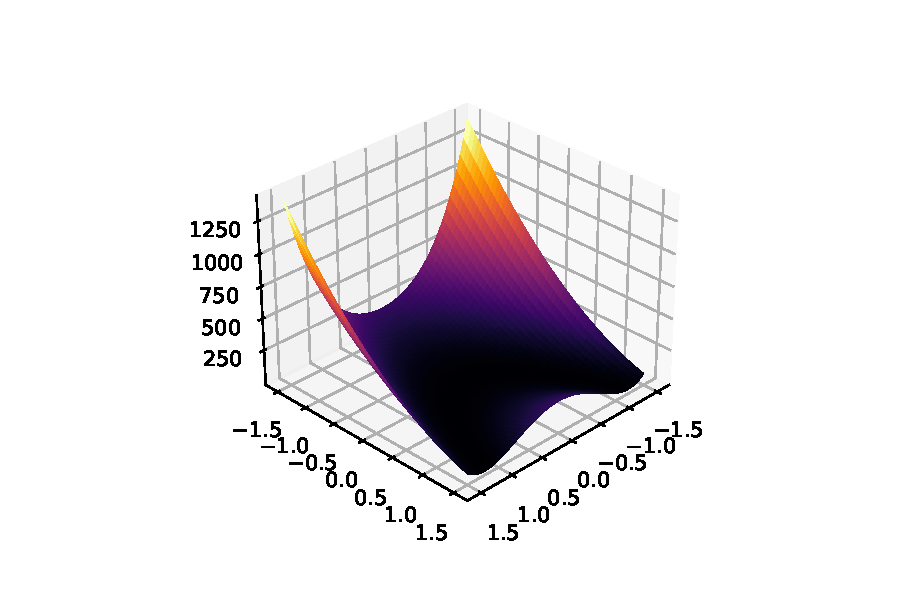
\includegraphics[width=1.5\textwidth,scale=3, trim=3.5cm 0 0 0]{assets/rosenbrock.pdf}
        \caption{Розенброка}
    \end{subfigure}
    \begin{subfigure}{0.3 \textwidth}
        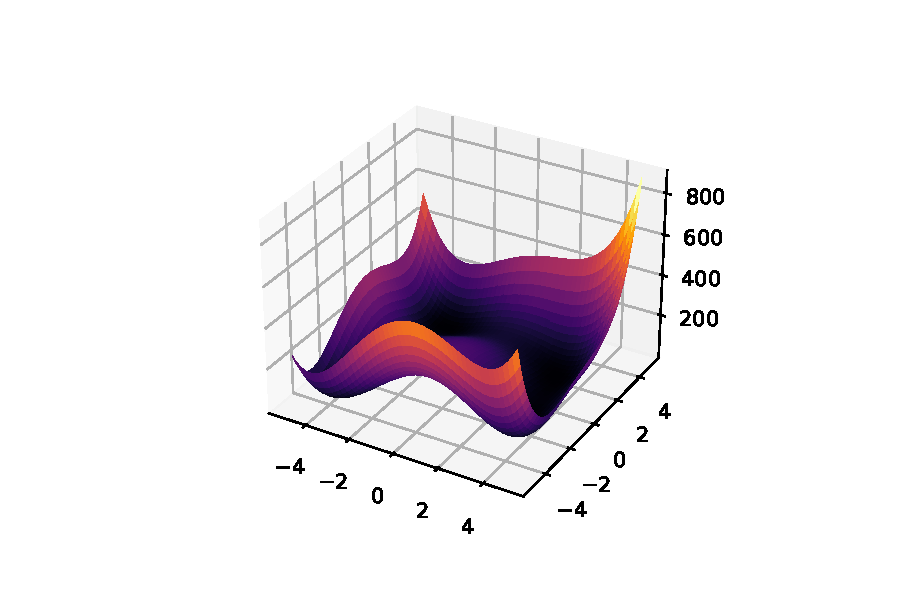
\includegraphics[width=1.45\textwidth, scale=3, trim=3.5cm 0 0 0]{assets/himmelblau.pdf}
        \caption{Хіммельблау}
    \end{subfigure}
    \begin{subfigure}{0.3 \textwidth}
        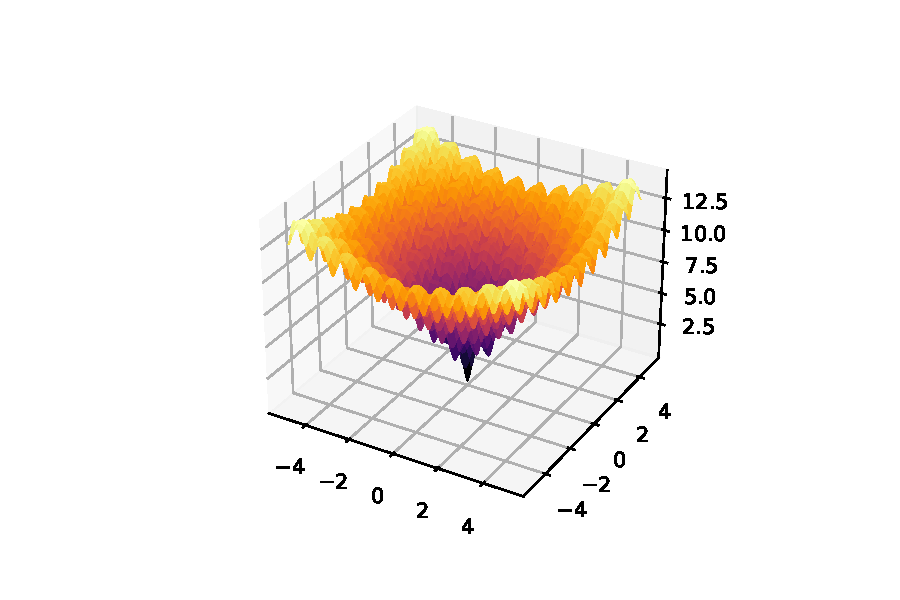
\includegraphics[width=1.5\textwidth, scale=3, trim=3.5cm 0 0 0]{assets/ackley.pdf}
        \caption{Еклі}
    \end{subfigure}
\end{figure}

\begin{enumerate}
    \item Функція Розенброка
    $$ f(x) = 100(x_2-x_1^2)^2 + (x_1-1)^2 $$
    \item Функція Хіммельблау
    $$ f(x) = (x_1^2 + x_2 - 11)^2 + (x_1 + x_2^2 - 7)^2 $$
    \item Функція Еклі
    $$ f(x) = -20 \exp{\left[-\frac{1}{5} \sqrt{\frac{x_1^2 + x_2^2}{2}}\right]} -
    \exp{\left[\frac{\cos(2 \pi x_1) + \cos(2 \pi x_2)}{2}\right]} + e + 20 $$
\end{enumerate}

\clearpage
\begin{table}[h!]
    \centering
    \begin{tabular}{|c|c|c|}
        \hline
        Функція & $x_{min}$ & $f(x_{min})$ \\
        \hline
        Розенброка & (1, 1) &
        \multirow{6}{*}{0} \\ \cline{1-2}

        \multirow{4}{*}{Хіммельблау} &
        (3, 2) & \\ \cline{2-2}
        & $\approx$ (-2.8, 3.13) &  \\ \cline{2-2}
        & $\approx$ (-3.78, -3.28) &  \\ \cline{2-2}
        & $\approx$ (3.58, -1.85) &  \\ \cline{1-2}

        Еклі & (0, 0) & \\
        \hline
    \end{tabular}
    \caption{Мінімуми досліджуваних функцій}
\end{table}

\subsection*{Метод Нелдера-Міда}

\begin{figure}[h!]
    \begin{subfigure}{0.5\textwidth}
        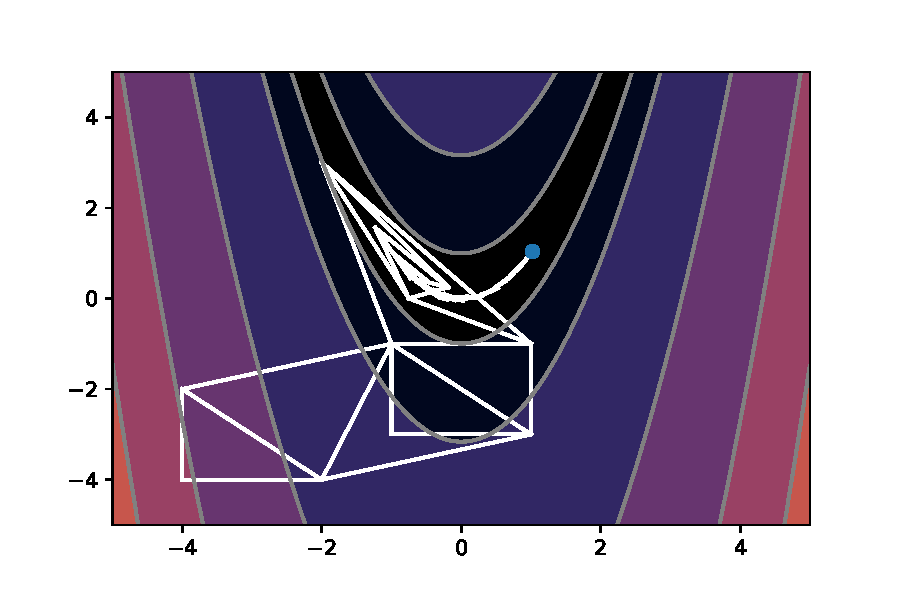
\includegraphics[width=\textwidth, trim=1cm 0.5cm 1.3cm 1cm, clip]{assets/NelderMead/rosenbrock.pdf}
        \caption{Розенброка}
    \end{subfigure}
    \begin{subfigure}{0.5\textwidth}
        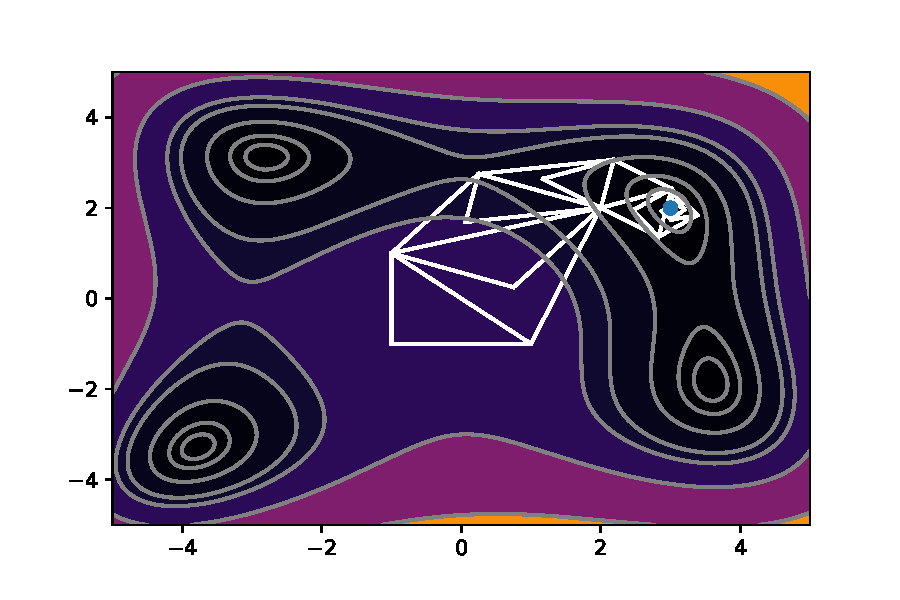
\includegraphics[width=\textwidth, trim=1cm 0.5cm 1.3cm 1cm, clip]{assets/NelderMead/himmelblau.pdf}
        \caption{Хіммельблау}
    \end{subfigure}
    \begin{subfigure}{\textwidth}
        \centering
        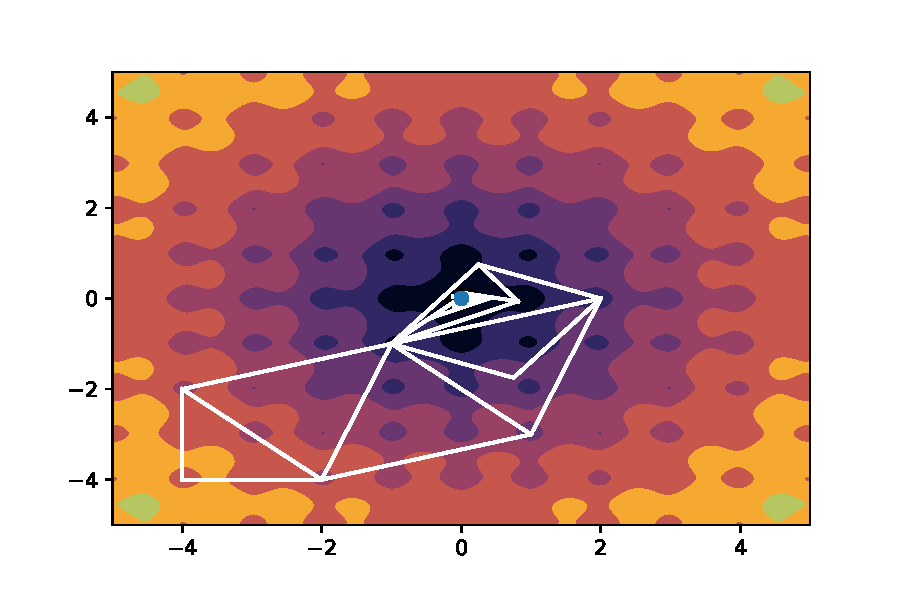
\includegraphics[width=0.5\textwidth, trim=1cm 0.5cm 1.3cm 1cm, clip]{assets/NelderMead/ackley.pdf}
        \caption{Еклі}
    \end{subfigure}
    \caption{Результати запуску методу Нелдера-Міда на функції}
\end{figure}

\pagebreak
\subsection*{Метод Гука-Дживса}

\begin{figure}[h!]
    \begin{subfigure}{0.5\textwidth}
        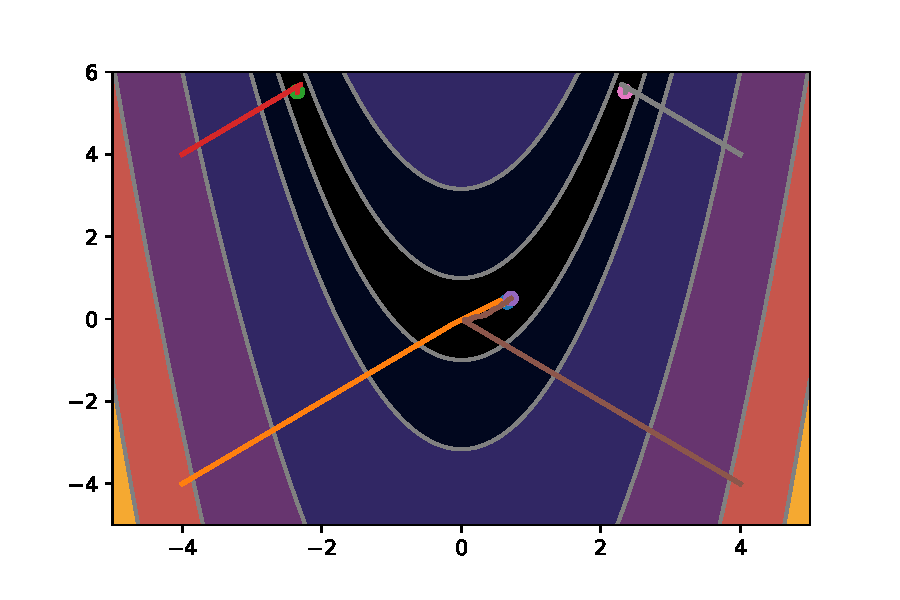
\includegraphics[width=\textwidth, trim=1cm 0.5cm 1.3cm 1cm, clip]{assets/HookeJeeves/rosenbrock.pdf}
        \caption{Розенброка}
    \end{subfigure}
    \begin{subfigure}{0.5\textwidth}
        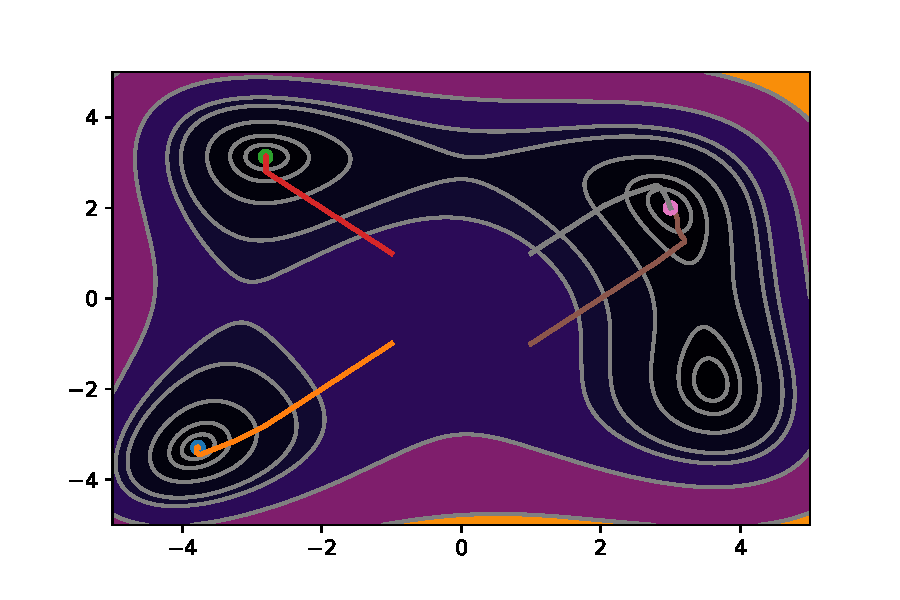
\includegraphics[width=\textwidth, trim=1cm 0.5cm 1.3cm 1cm, clip]{assets/HookeJeeves/himmelblau.pdf}
        \caption{Хіммельблау}
    \end{subfigure}
    \begin{subfigure}{\textwidth}
        \centering
        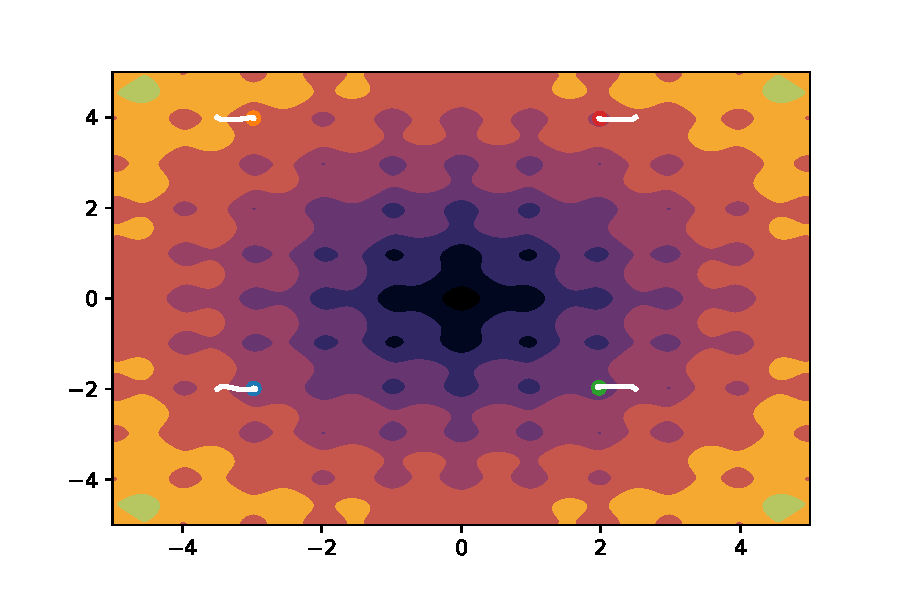
\includegraphics[width=0.5\textwidth, trim=1cm 0.5cm 1.3cm 1cm, clip]{assets/HookeJeeves/ackley.pdf}
        \caption{Еклі}
    \end{subfigure}
    \caption{Результати запуску методу Гука-Дживса на функції}
\end{figure}

\subsection*{Метод Ньютона}

\begin{figure}[h!]
    \begin{subfigure}{0.5\textwidth}
        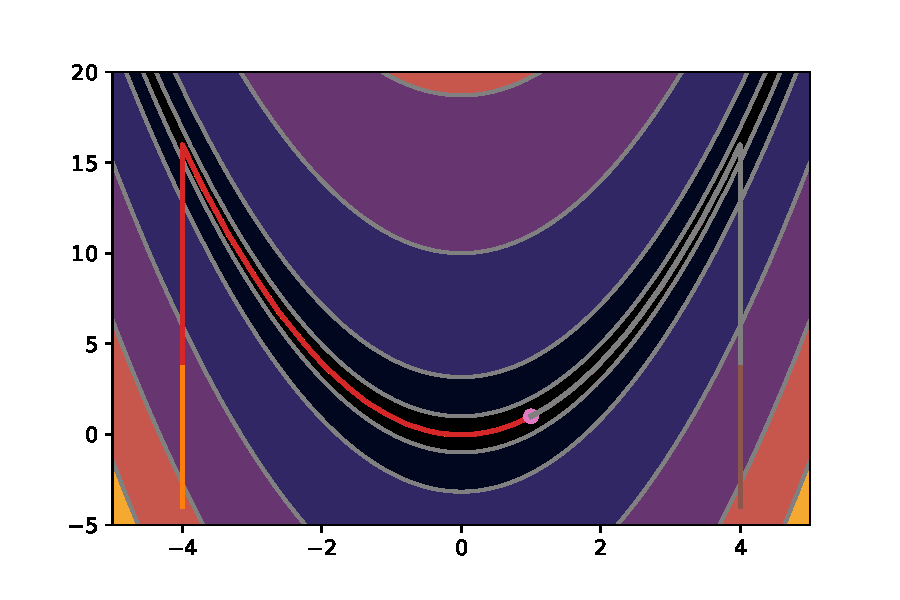
\includegraphics[width=\textwidth, trim=1cm 0.5cm 1.3cm 1cm, clip]{assets/Newton/rosenbrock.pdf}
        \caption{Розенброка}
    \end{subfigure}
    \begin{subfigure}{0.5\textwidth}
        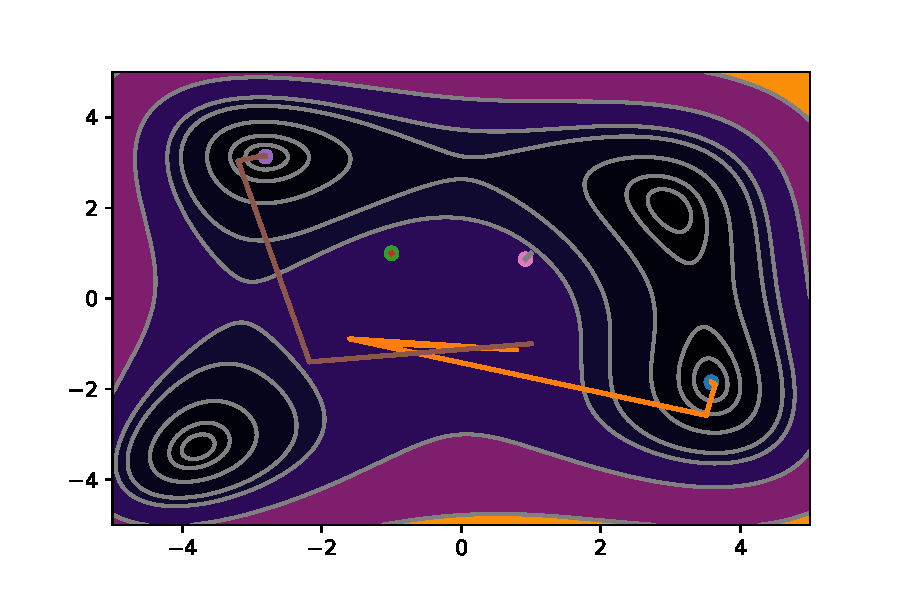
\includegraphics[width=\textwidth, trim=1cm 0.5cm 1.3cm 1cm, clip]{assets/Newton/himmelblau.pdf}
        \caption{Хіммельблау}
    \end{subfigure}
\end{figure}
\begin{figure}[h!]
    \ContinuedFloat
    \begin{subfigure}{\textwidth}
        \centering
        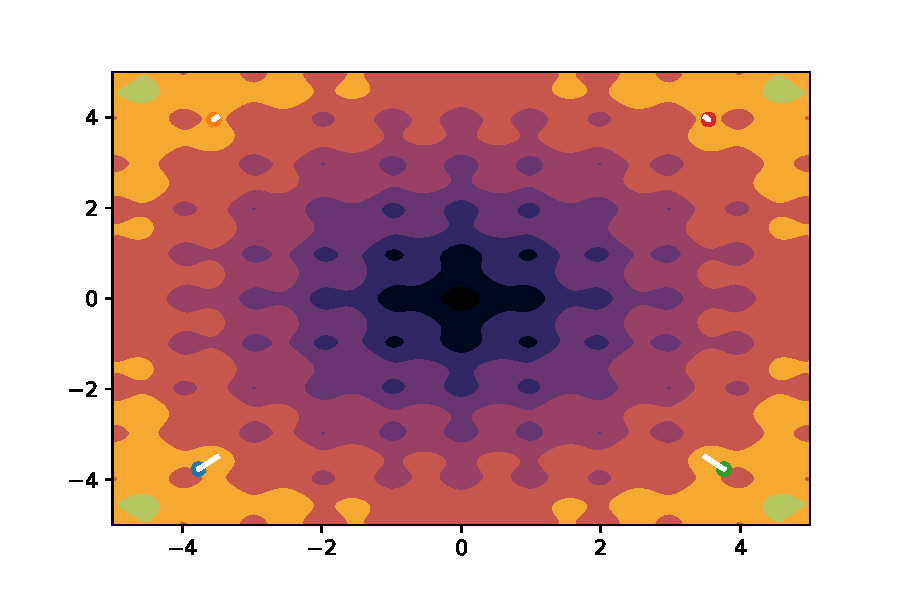
\includegraphics[width=0.5\textwidth, trim=1cm 0.5cm 1.3cm 1cm, clip]{assets/Newton/ackley.pdf}
        \caption{Еклі}
    \end{subfigure}
    \caption{Результати запуску методу Ньютона на функції}
\end{figure}

\pagebreak
\subsection*{Квазіньютоновські методи}

\begin{figure}[h!]
    \begin{subfigure}{0.5\textwidth}
        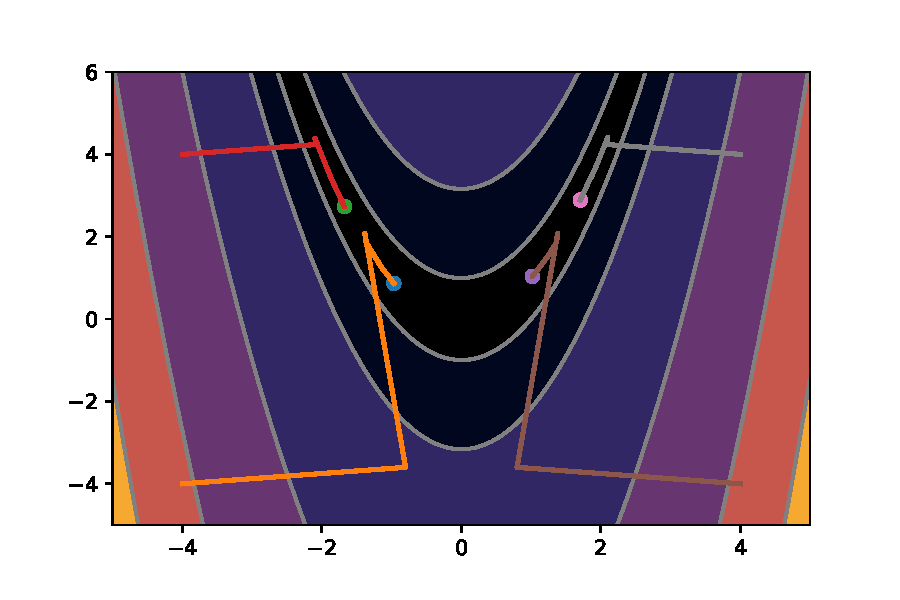
\includegraphics[width=\textwidth, trim=1cm 0.5cm 1.3cm 1cm, clip]{assets/SR1/rosenbrock.pdf}
        \caption{SR1}
    \end{subfigure}
    \begin{subfigure}{0.5\textwidth}
        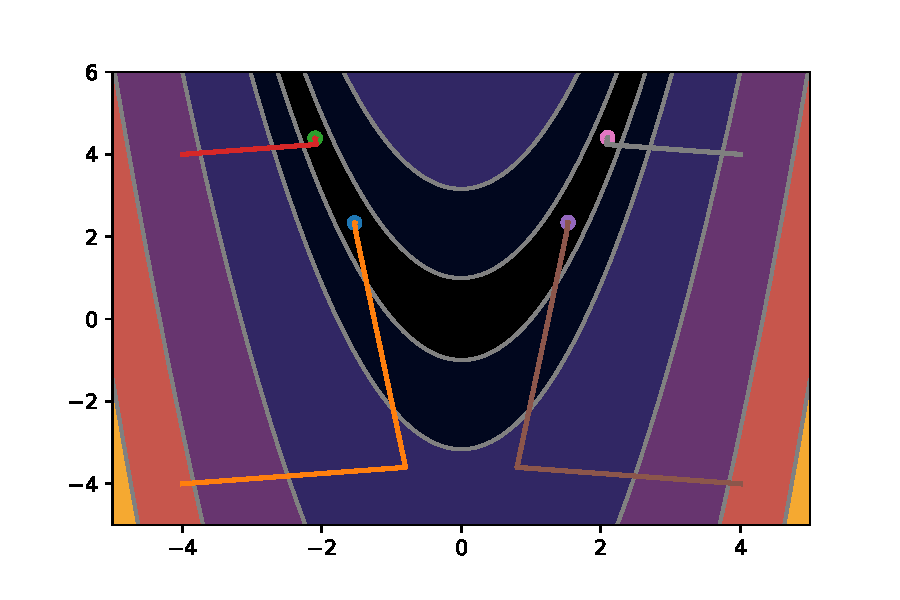
\includegraphics[width=\textwidth, trim=1cm 0.5cm 1.3cm 1cm, clip]{assets/Broyden/rosenbrock.pdf}
        \caption{Broyden}
    \end{subfigure}
    \begin{subfigure}{0.5\textwidth}
        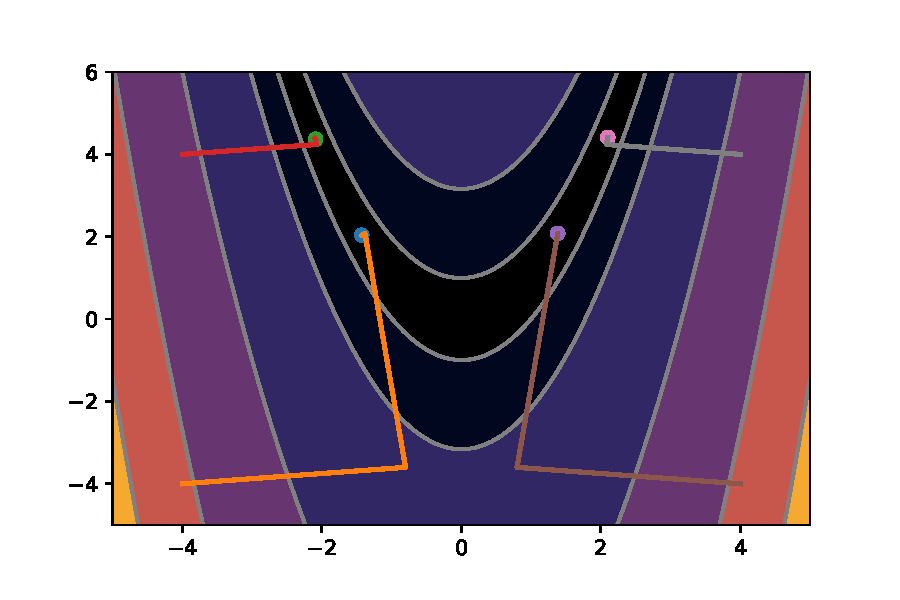
\includegraphics[width=\textwidth, trim=1cm 0.5cm 1.3cm 1cm, clip]{assets/DFP/rosenbrock.pdf}
        \caption{DFP}
    \end{subfigure}
    \begin{subfigure}{0.5\textwidth}
        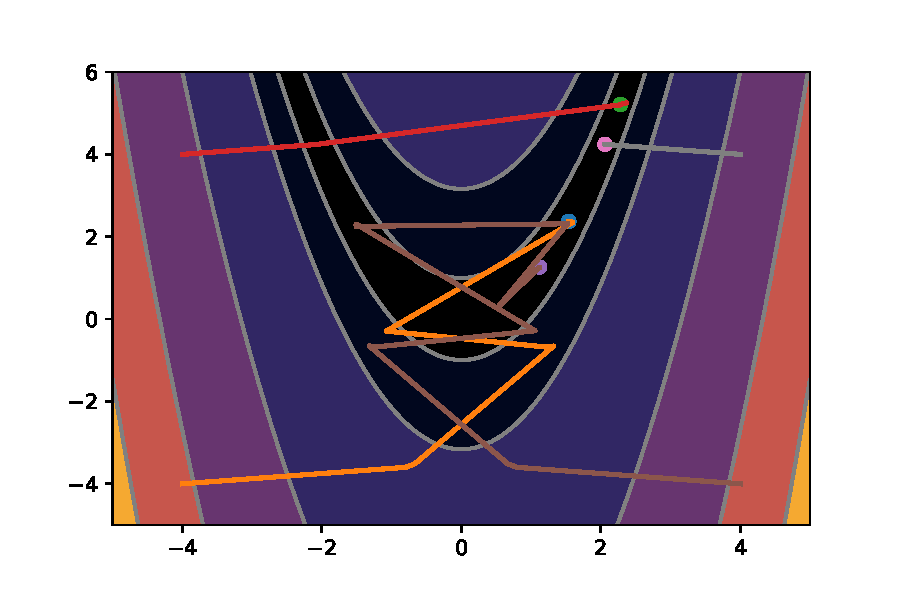
\includegraphics[width=\textwidth, trim=1cm 0.5cm 1.3cm 1cm, clip]{assets/BFGS/rosenbrock.pdf}
        \caption{BFGS}
    \end{subfigure}
    \caption{Результати запуску квазіньютоновських методів на функції Розенброка}
\end{figure}

\begin{figure}[h!]
    \begin{subfigure}{0.5\textwidth}
        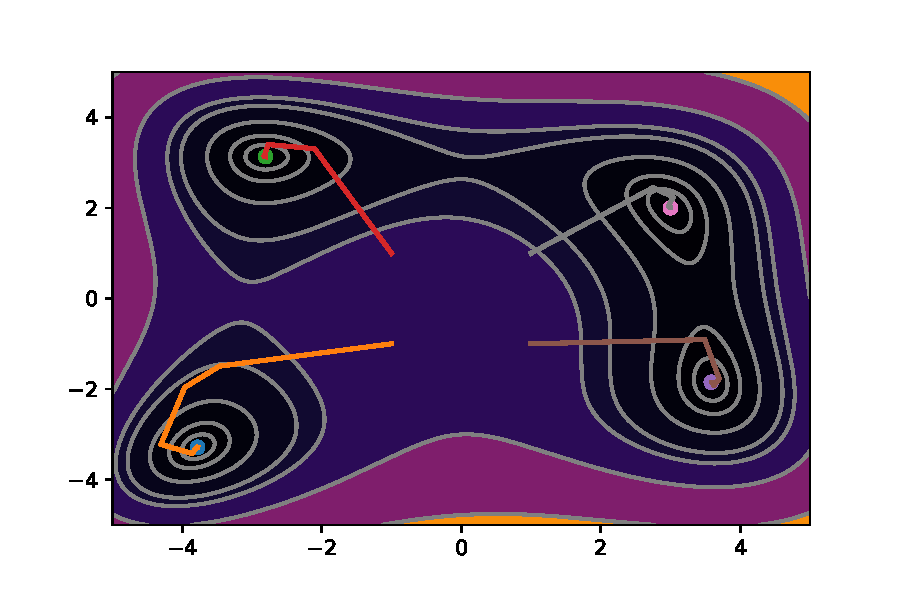
\includegraphics[width=\textwidth, trim=1cm 0.5cm 1.3cm 1cm, clip]{assets/SR1/himmelblau.pdf}
        \caption{SR1}
    \end{subfigure}
    \begin{subfigure}{0.5\textwidth}
        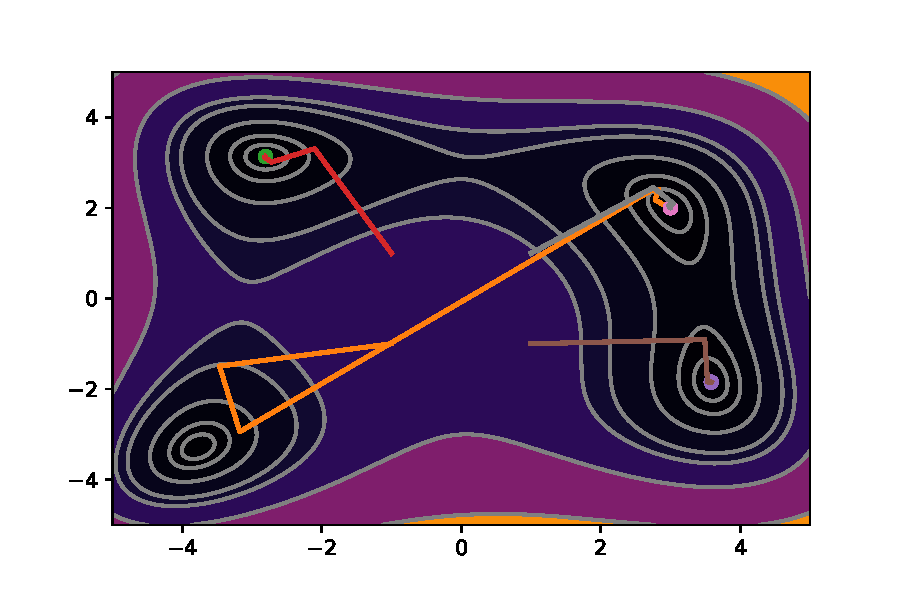
\includegraphics[width=\textwidth, trim=1cm 0.5cm 1.3cm 1cm, clip]{assets/Broyden/himmelblau.pdf}
        \caption{Broyden}
    \end{subfigure}
    \begin{subfigure}{0.5\textwidth}
        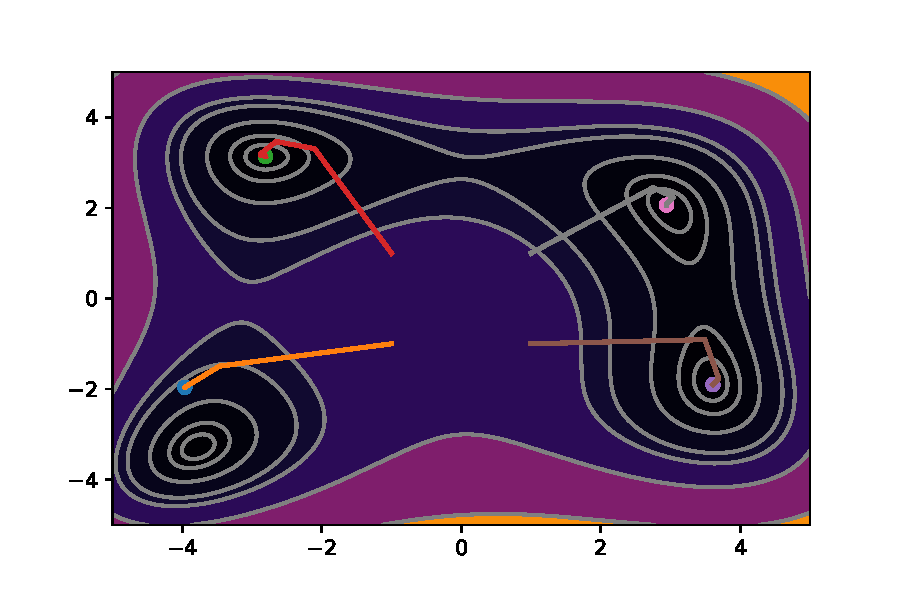
\includegraphics[width=\textwidth, trim=1cm 0.5cm 1.3cm 1cm, clip]{assets/DFP/himmelblau.pdf}
        \caption{DFP}
    \end{subfigure}
    \begin{subfigure}{0.5\textwidth}
        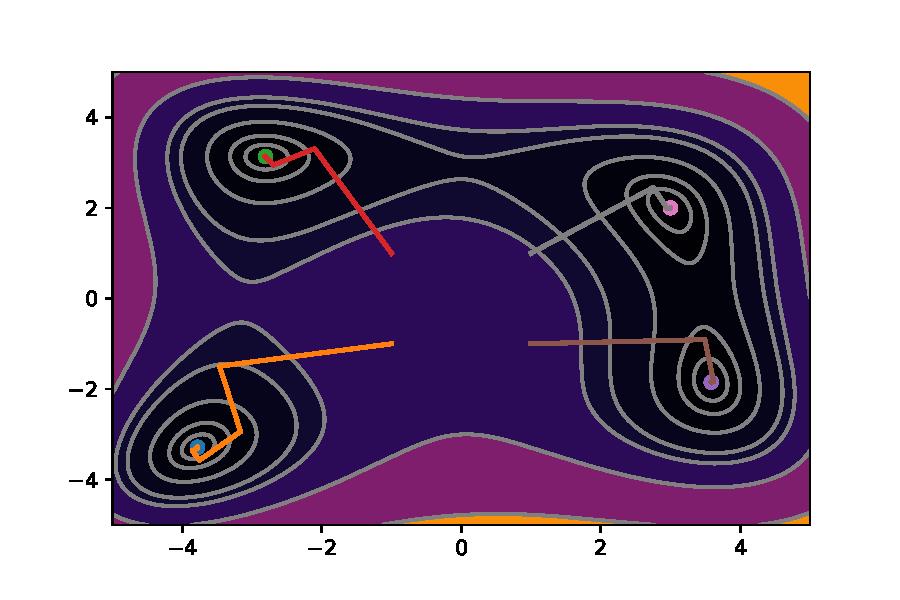
\includegraphics[width=\textwidth, trim=1cm 0.5cm 1.3cm 1cm, clip]{assets/BFGS/himmelblau.pdf}
        \caption{BFGS}
    \end{subfigure}
    \caption{Результати запуску квазіньютоновських методів на функції Хіммельблау}
\end{figure}

\begin{figure}[h!]
    \begin{subfigure}{0.5\textwidth}
        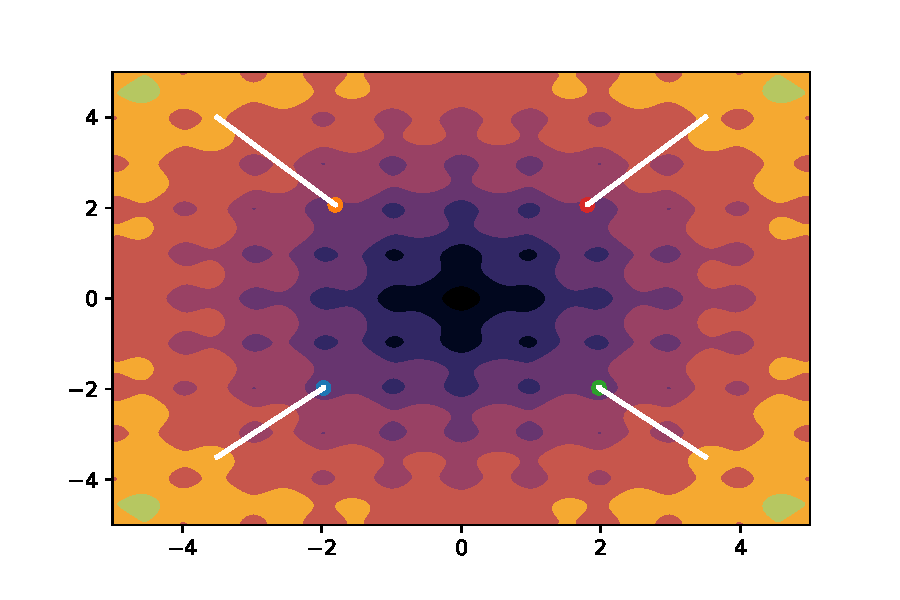
\includegraphics[width=\textwidth, trim=1cm 0.5cm 1.3cm 1cm, clip]{assets/SR1/ackley.pdf}
        \caption{SR1}
    \end{subfigure}
    \begin{subfigure}{0.5\textwidth}
        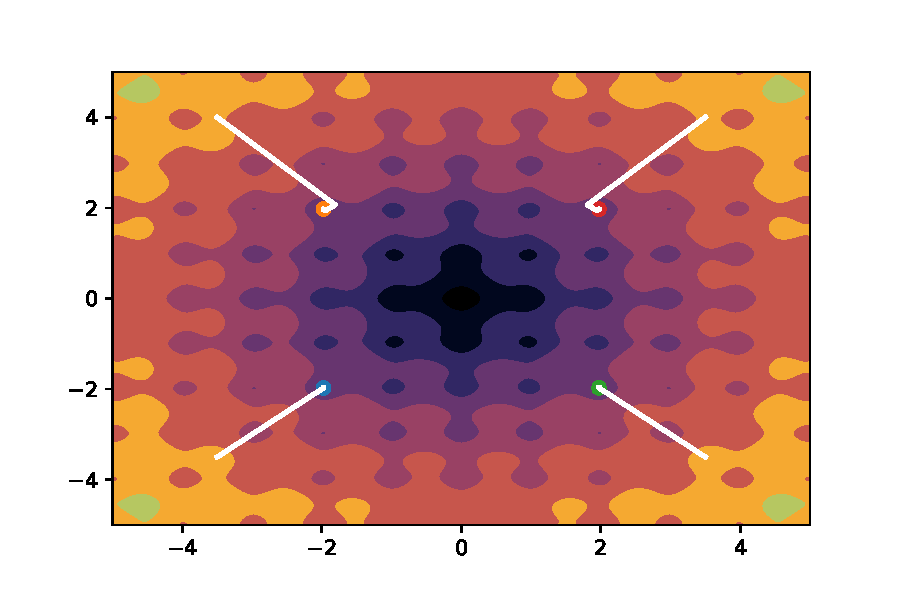
\includegraphics[width=\textwidth, trim=1cm 0.5cm 1.3cm 1cm, clip]{assets/Broyden/ackley.pdf}
        \caption{Broyden}
    \end{subfigure}
\end{figure}
\begin{figure}
    \ContinuedFloat
    \begin{subfigure}{0.5\textwidth}
        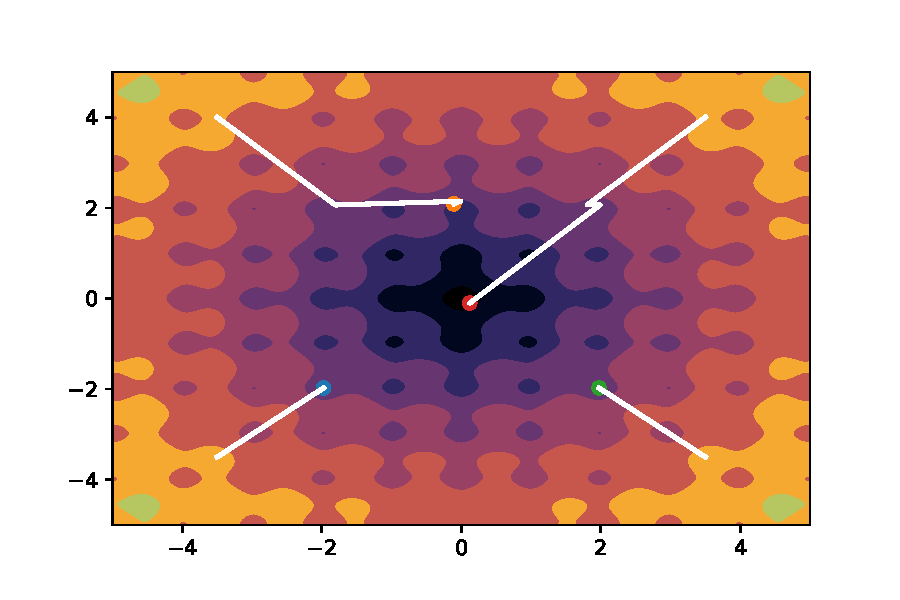
\includegraphics[width=\textwidth, trim=1cm 0.5cm 1.3cm 1cm, clip]{assets/DFP/ackley.pdf}
        \caption{DFP}
    \end{subfigure}
    \begin{subfigure}{0.5\textwidth}
        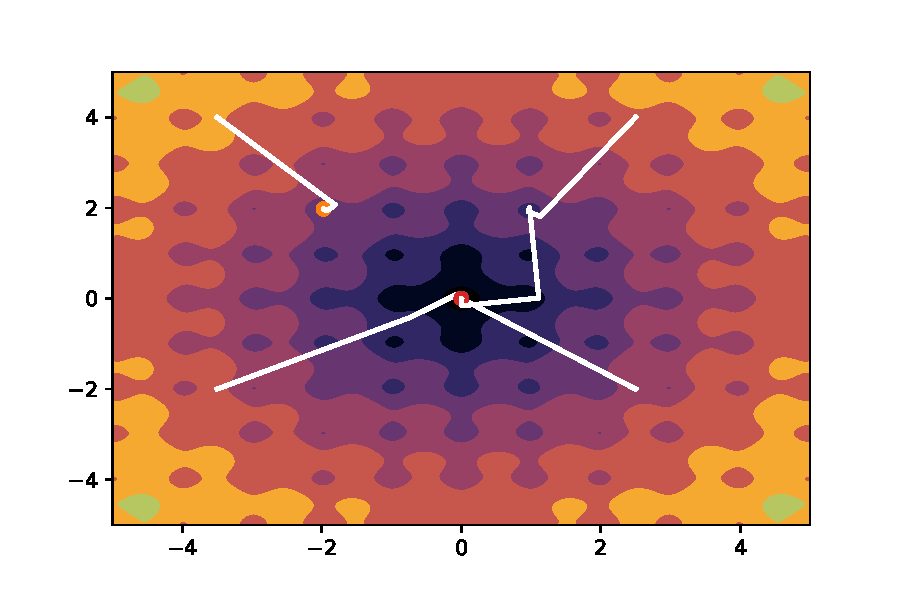
\includegraphics[width=\textwidth, trim=1cm 0.5cm 1.3cm 1cm, clip]{assets/BFGS/ackley.pdf}
        \caption{BFGS}
    \end{subfigure}
    \caption{Результати запуску квазіньютоновських методів на функції Еклі}
\end{figure}

\vspace*{10cm}
\subsection*{Генетичний алгоритм}

\pagebreak
\subsection*{Порівняння досліджуваних методів оптимізації}
Для порівняння усіх імплементованих у цій роботі методів,
пободуємо таблиці з результатами запусків алгоритмів з 4
різних початкових умов.

\subsubsection*{Метод Нелдера-Міда}
Початковий симплекс для методів Нелдера-Міда ми обирали наступним чином:
була вибрана початкова точка $x_0$ та параметр $l \in \mathbb{R}$.
Кожна наступна $i$-та точка симплекса була обчислена шляхом додавання
до $i$-той координати $x_0$ величини $l$. За критерій зупинки
було обрано наступне: стандартне відхилення значень функції
у кожній точці симплекса менше за $10^{-3}$.

\begin{table}[h!]
    \centering
    \begin{tabular}{|c|c|c|c|c|}
        \hline
        \textbf{Функція} & \textbf{Початковий симплекс} & $\approx x_{res}$ & $\approx f(x_{res})$ & \textbf{Кількість ітерацій}  \\
        \hline
        Розенброка & (-4,-4) (-4, -2) (-2, -4) & (1.02, 1.04) & 0.01 & 65
        \\ \hline
        Хіммельблау & (-1,-1) (-1, 1) (1, -1) & (3,2) & 0 & 25
        \\ \hline
        Еклі & (-4,-4) (-4, -2) (-2, -4) & (0, 0) & 0 & 26
        \\ \hline
    \end{tabular}
    \caption{Результати запусків методу Нелдера-Міда}
\end{table}

\subsubsection*{Метод Гука-Дживса}

Наведемо результати запуску алгорима Гука-Дживса
з різних початкових точок.
Умовою зупинки для усіх варіацій була
умова $\Delta f(x) < 10^{-3}$.

\begin{table}[h!]
    \centering
    \begin{tabular}{|c|c|c|c|c|c|}
        \hline
        \textbf{Функція} & $x_0$ & $\approx x_{res}$ & $\approx f(x_{res})$ & \textbf{Кількість ітерацій}  \\
        \hline
        \multirow{4}{*}{Розенброка} & (-4 , -4) & (0.66,0.42) & 4.31 & 25 \\
        \cline{2-5}
        & (-4, 4) & (-2.35,5.52) & 13.7 & 13 \\
        \cline{2-5}
        & (4, -4) & (0.71,0.5) & 4.5 & 38 \\
        \cline{2-5}
        & (4, 4) & (2.35,5.52) & 13.7 & 13 \\
        \hline
        \multirow{4}{*}{Хіммельблау} & (-1 , -1) & (-3.77,-3.29) & 0.0 & 14 \\
        \cline{2-5}
        & (-1 , 1) & (-2.8,3.13) & 0.0 & 15 \\
        \cline{2-5}
        & (1 , -1) & (3.0,2.0) & 0.0 & 16 \\
        \cline{2-5}
        & (1 , 1) & (3.0,2.0) & 0.0 & 13 \\
        \hline
        \multirow{4}{*}{Еклі} & (-3.5, 2) & (-2.98,-1.99) & 7.96 & 7 \\
        \cline{2-5}
        & (-3.5, 4) & (-2.98,3.98) & 10.12 & 7
        \\ \cline{2-5}
        & (2.5, 2) &(1.97,-1.97) & 6.56 & 7
        \\ \cline{2-5}
        & (2.5, 4) & (1.99,3.97) & 9.35 & 7
        \\ \hline
    \end{tabular}
    \caption{Результати запусків методу Гука-Дживса}
\end{table}

\subsubsection*{Методи типу Ньютона}

Усі наступні [квазі]ньютоновські методи використовували
метод перебору для пошуку розміру кроку, та
комбінований критерій зупинки:
або $\Delta x_k < 0.5 \cdot 10^{-3}$,
або $\nabla f_k < 10^{-4}$.

\vspace{-0.21cm}
\begin{table}[h!]
    \centering
    \begin{tabular}{|c|c|c|c|c|}
        \hline
        \textbf{Алгоритм} & $x_{0}$ & $\approx x_{res}$ & $\approx f(x_{res})$ & \textbf{Кількість ітерацій}  \\
        \hline
        Newton & \multirow{5}{*}{(-4,-4)} & (1.0,1.0) & 0 & 24 \\
        \cline{1-1} \cline{3-5}
        SR1 & & (-1.68,2.73) & 4.32 & 6 \\
        \cline{1-1} \cline{3-5}
        Broyden & & (-2.1,4.39) & 6.39 & 4 \\
        \cline{1-1} \cline{3-5}
        DFP & & (-2.09,4.37) & 5.89 & 5 \\
        \cline{1-1} \cline{3-5}
        BFGS & & (2.28,5.21) & 0.29 & 13 \\
        \hline
        Newton & \multirow{5}{*}{(-4,4)} & (1.0,1.0) & 0 & 24 \\
        \cline{1-1} \cline{3-5}
        SR1 & & (-1.68,2.73) & 7.73 & 6 \\
        \cline{1-1} \cline{3-5}
        Broyden & & (-2.1,4.39) & 9.58 & 4 \\
        \cline{1-1} \cline{3-5}
        DFP & & (-2.09,4.37) & 9.55 & 5 \\
        \cline{1-1} \cline{3-5}
        BFGS & & (2.28,5.21) & 1.64 & 13 \\
        \hline
        Newton & \multirow{5}{*}{(4,-4)} & (1.0,1.0) & 0 & 18 \\
        \cline{1-1} \cline{3-5}
        SR1 & & (1.02,1.04) & 0 & 11 \\
        \cline{1-1} \cline{3-5}
        Broyden & & (1.53,2.35) & 0.28 & 4 \\
        \cline{1-1} \cline{3-5}
        DFP & & (1.38,2.08) & 3 & 3 \\
        \cline{1-1} \cline{3-5}
        BFGS & & (1.12,1.26) & 0.02 & 30 \\
        \hline
        Newton & \multirow{5}{*}{(4,4)} & (1.0,1.0) & 0 & 18 \\
        \cline{1-1} \cline{3-5}
        SR1 & & (1.71,2.89) & 0.56 & 8 \\
        \cline{1-1} \cline{3-5}
        Broyden & & (2.1,4.41) & 1.21 & 4 \\
        \cline{1-1} \cline{3-5}
        DFP & & (2.1,4.41) & 1.21 & 3 \\
        \cline{1-1} \cline{3-5}
        BFGS & & (2.06,4.24) & 1.12 & 9 \\
        \hline
    \end{tabular}
    \caption{Порівняльна таблиця для функції Розенброка}
\end{table}

\vspace{-0.8cm}
\begin{table}[h!]
    \centering
    \begin{tabular}{|c|c|c|c|c|}
        \hline
        \textbf{Алгоритм} & $x_{0}$ & $\approx x_{res}$ & $\approx f(x_{res})$ & \textbf{Кількість ітерацій}  \\
        \hline
        Newton & \multirow{5}{*}{(-1,-1)} & (3.58,-1.85) & 0 & 6 \\
        \cline{1-1} \cline{3-5}
        SR1 & & (-3.78,-3.28) & 0 & 7 \\
        \cline{1-1} \cline{3-5}
        Broyden & & (3.0,2.0) & 0 & 9 \\
        \cline{1-1} \cline{3-5}
        DFP & & (-3.96,-1.96) & 58.27 & 3 \\
        \cline{1-1} \cline{3-5}
        BFGS & & (-3.78,-3.28) & 0 & 10 \\
        \cline{1-1} \cline{3-5}
        \hline
        Newton & \multirow{5}{*}{(-1, 1)} & (-1.0,1.0) & 130.01 & 1 \\
        \cline{1-1} \cline{3-5}
        SR1 & & (-2.81,3.13) & 0 & 6 \\
        \cline{1-1} \cline{3-5}
        Broyden & & (-2.81,3.13) & 0 & 5 \\
        \cline{1-1} \cline{3-5}
        DFP & & (-2.81,3.13) & 0 & 67 \\
        \cline{1-1} \cline{3-5}
        BFGS & & (-2.81,3.13) & 0 & 6 \\
        \hline
        Newton & \multirow{5}{*}{(1, -1)} & (-2.81,3.13) & 0 & 5 \\
        \cline{1-1} \cline{3-5}
        SR1 & & (3.58,-1.85) & 0 & 6 \\
        \cline{1-1} \cline{3-5}
        Broyden & & (3.58,-1.85) & 0 & 6 \\
        \cline{1-1} \cline{3-5}
        DFP & & (3.61,-1.9) & 0.06 & 4 \\
        \cline{1-1} \cline{3-5}
        BFGS & & (3.58,-1.85) & 0 & 7 \\
        \hline
        Newton & \multirow{5}{*}{(1, 1)} & (0.92,0.87) & 114.51 & 250 \\
        \cline{1-1} \cline{3-5}
        SR1 & & (3.0,2.0) & 0 & 6 \\
        \cline{1-1} \cline{3-5}
        Broyden & & (3.0,2.0) & 0 & 6 \\
        \cline{1-1} \cline{3-5}
        DFP & & (2.94,2.06) & 0.11 & 5 \\
        \cline{1-1} \cline{3-5}
        BFGS & & (3.0,2.0) & 0 & 6 \\
        \hline
    \end{tabular}
    \caption{Порівняльна таблиця для функції Хіммельблау}
\end{table}

\clearpage
\begin{table}[ht!]
    \centering
    \begin{tabular}{|c|c|c|c|c|}
        \hline
        \textbf{Алгоритм} & $x_{0}$ & $\approx x_{res}$ & $\approx f(x_{res})$ & \textbf{Кількість ітерацій}  \\
        \hline
        Ньютона & \multirow{5}{*}{(-3.5, 2)} & (-3.5,-2.0) & 10.41 & 1 \\
        \cline{1-1} \cline{3-5}
        SR1 & & (-1.06,-0.89) & 3.95 & 4 \\
        \cline{1-1} \cline{3-5}
        Broyden & & (-0.0,0.95) & 2.58 & 5 \\
        \cline{1-1} \cline{3-5}
        DFP & & (0.12,-0.2) & 1.71 & 5 \\
        \cline{1-1} \cline{3-5}
        BFGS & & (0.0,0.0) & 0.0 & 7 \\
        \hline
        Ньютона & \multirow{5}{*}{(-3.5, 4)} & (-3.55,3.95) & 12.28 & 3 \\
        \cline{1-1} \cline{3-5}
        SR1 & & (-1.81,2.06) & 7.27 & 2 \\
        \cline{1-1} \cline{3-5}
        Broyden & & (-1.97,1.97) & 6.56 & 5 \\
        \cline{1-1} \cline{3-5}
        DFP & & (-0.11,2.09) & 5.58 & 5 \\
        \cline{1-1} \cline{3-5}
        BFGS & & (-1.97,1.97) & 6.56 & 6 \\
        \hline
        Newton & \multirow{5}{*}{(2.5, -2)} & (2.5,-2.0) & 9.0 & 1 \\
        \cline{1-1} \cline{3-5}
        SR1 & & (0.0,-0.0) & 0.0 & 4 \\
        \cline{1-1} \cline{3-5}
        Broyden & & (0.0,0.0) & 0.0 & 4 \\
        \cline{1-1} \cline{3-5}
        DFP & & (0.0,-0.0) & 0.0 & 2 \\
        \cline{1-1} \cline{3-5}
        BFGS & & (0.0,-0.0) & 0.0 & 2 \\
        \hline
        Newton & \multirow{5}{*}{(2.5,4)} & (2.54,3.94) & 11.43 & 3 \\
        \cline{1-1} \cline{3-5}
        BFGS & & (1.97,1.97) & 6.56 & 6 \\
        \cline{1-1} \cline{3-5}
        SR1 & & (1.13,1.81) & 6.24 & 2 \\
        \cline{1-1} \cline{3-5}
        Broyden & & (0.98,1.96) & 5.38 & 6 \\
        \cline{1-1} \cline{3-5}
        DFP & & (1.13,1.81) & 6.24 & 2 \\
        \cline{1-1} \cline{3-5}
        BFGS & & (-0.0,0.0) & 0.0 & 13 \\
        \hline
    \end{tabular}
    \caption{Порівняльна таблиця для функції Еклі}
\end{table}
